\begin{figure*}[!hbt]
  \centering
  \subfigure[Runtime on consecutive batch updates of size $10^{-5}|E_T|$]{
    \label{fig:temporal-wiki-talk-temporal--runtime5}
    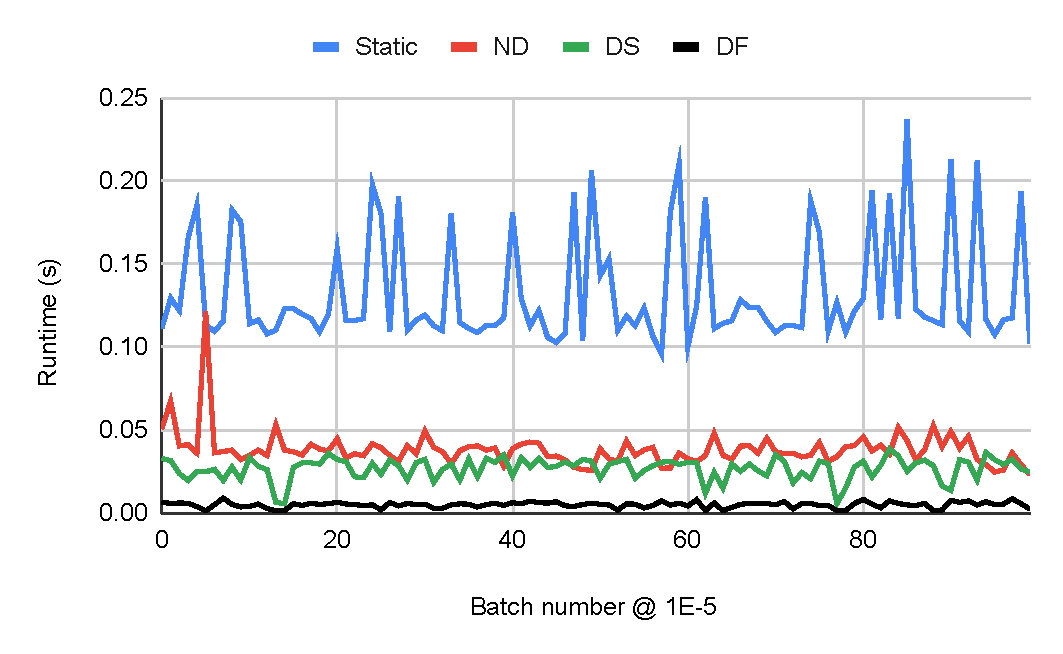
\includegraphics[width=0.48\linewidth]{out/temporal-wiki-talk-temporal-runtime5.pdf}
  }
  \subfigure[Modularity of communities obtained on consecutive batch updates of size $10^{-5}|E_T|$]{
    \label{fig:temporal-wiki-talk-temporal--modularity5}
    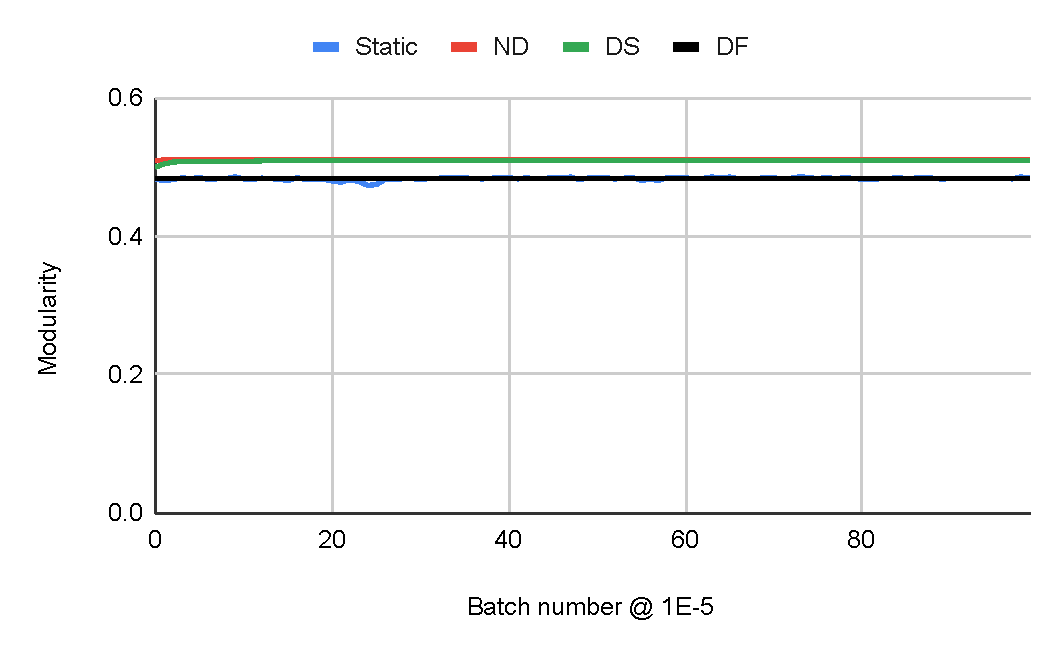
\includegraphics[width=0.48\linewidth]{out/temporal-wiki-talk-temporal-modularity5.pdf}
  } \\[2ex]
  \subfigure[Runtime on consecutive batch updates of size $10^{-4}|E_T|$]{
    \label{fig:temporal-wiki-talk-temporal--runtime4}
    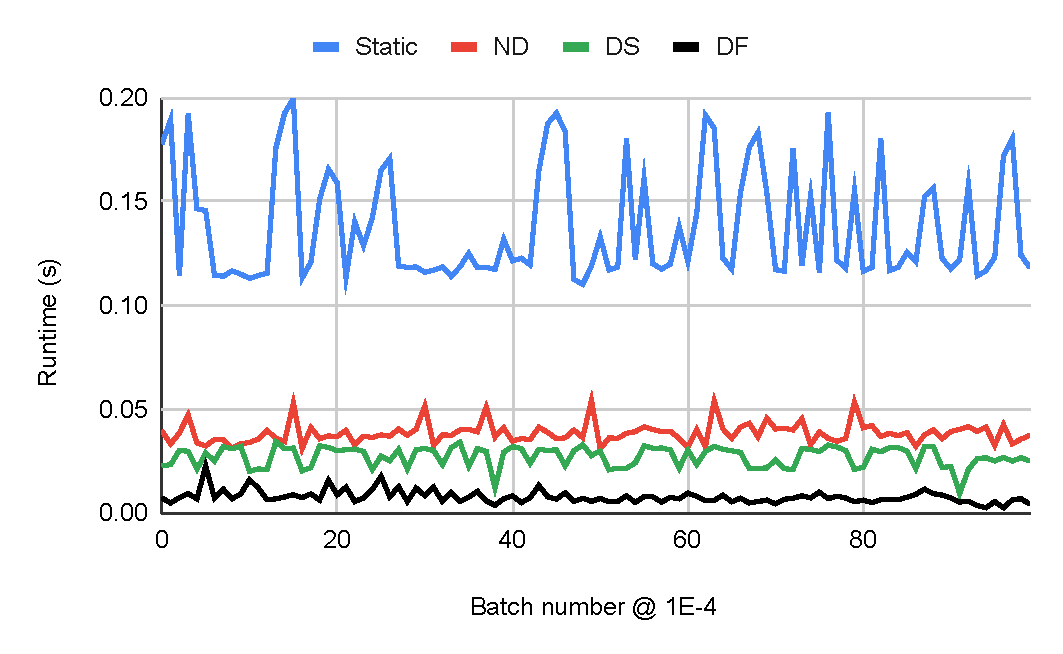
\includegraphics[width=0.48\linewidth]{out/temporal-wiki-talk-temporal-runtime4.pdf}
  }
  \subfigure[Modularity of communities obtained on consecutive batch updates of size $10^{-4}|E_T|$]{
    \label{fig:temporal-wiki-talk-temporal--modularity4}
    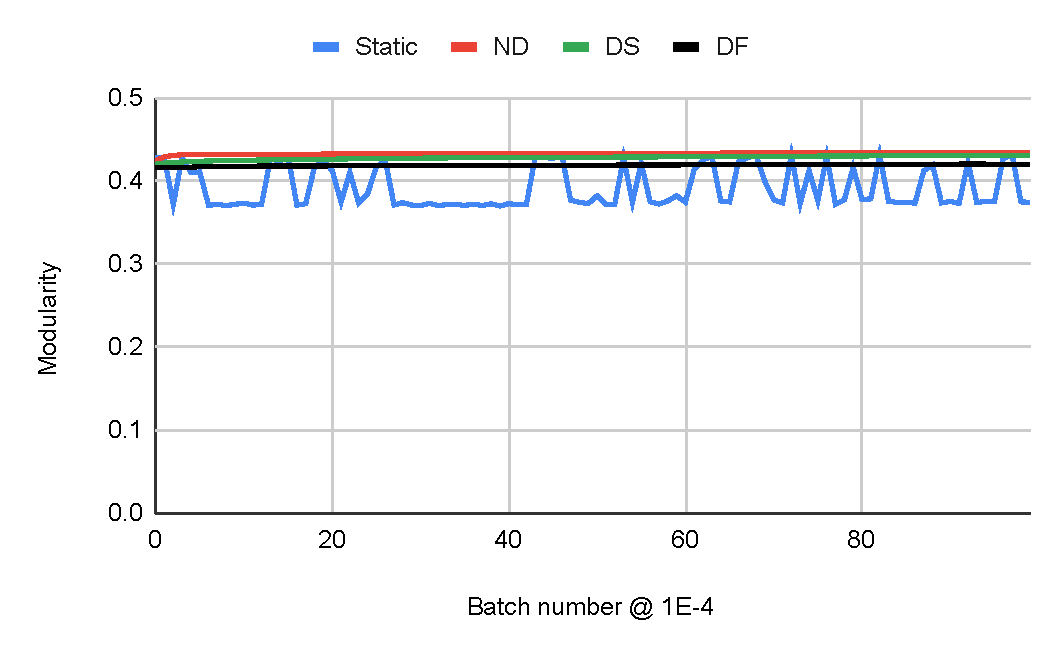
\includegraphics[width=0.48\linewidth]{out/temporal-wiki-talk-temporal-modularity4.pdf}
  } \\[2ex]
  \subfigure[Runtime on consecutive batch updates of size $10^{-3}|E_T|$]{
    \label{fig:temporal-wiki-talk-temporal--runtime3}
    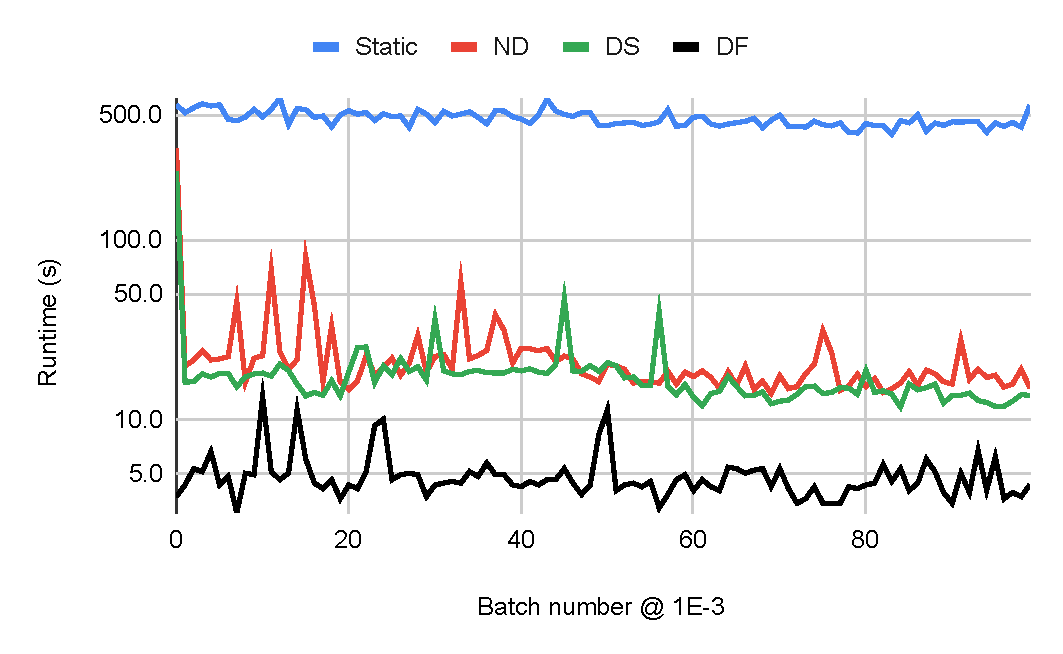
\includegraphics[width=0.48\linewidth]{out/temporal-wiki-talk-temporal-runtime3.pdf}
  }
  \subfigure[Modularity of communities obtained on consecutive batch updates of size $10^{-3}|E_T|$]{
    \label{fig:temporal-wiki-talk-temporal--modularity3}
    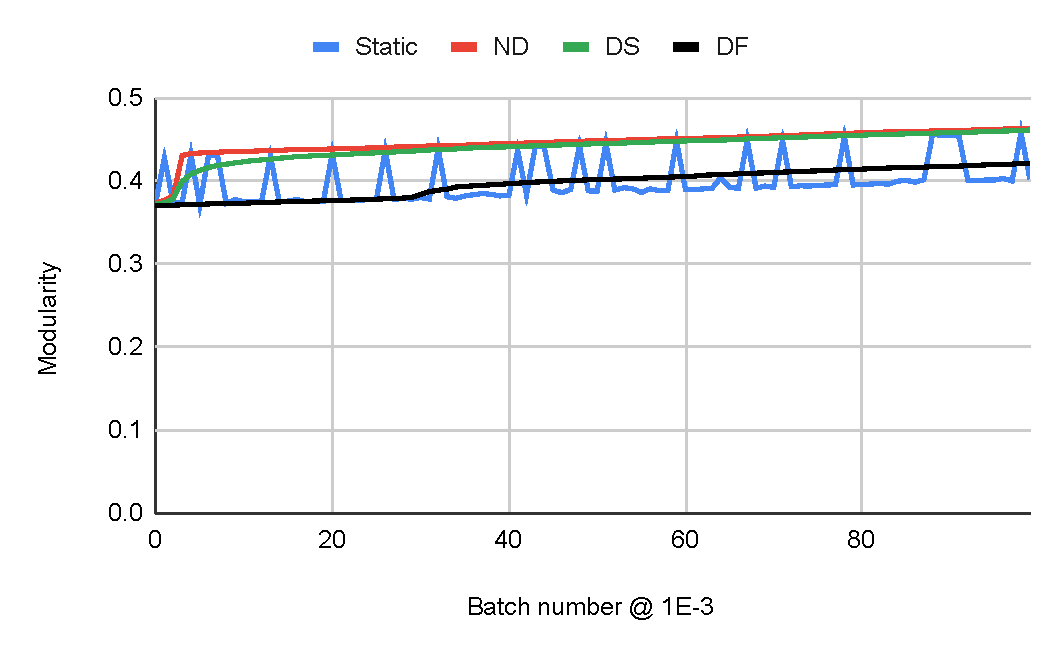
\includegraphics[width=0.48\linewidth]{out/temporal-wiki-talk-temporal-modularity3.pdf}
  } \\[-2ex]
  \caption{Runtime and Modularity of communities obtained with \textit{Static}, \textit{Naive-dynamic (ND)}, \textit{Delta-screening (DS)}, and \textit{Dynamic Frontier (DF)} Louvain on the \textit{wiki-talk-temporal} dynamic graph. The size of batch updates range from $10^{-5}|E_T|$ to $10^{-3}|E_T|$.}
  \label{fig:temporal-wiki-talk-temporal}
\end{figure*}
